\documentclass{standalone}

\usepackage{amsmath}
\usepackage{tikz}
\usetikzlibrary{math}

\begin{document}
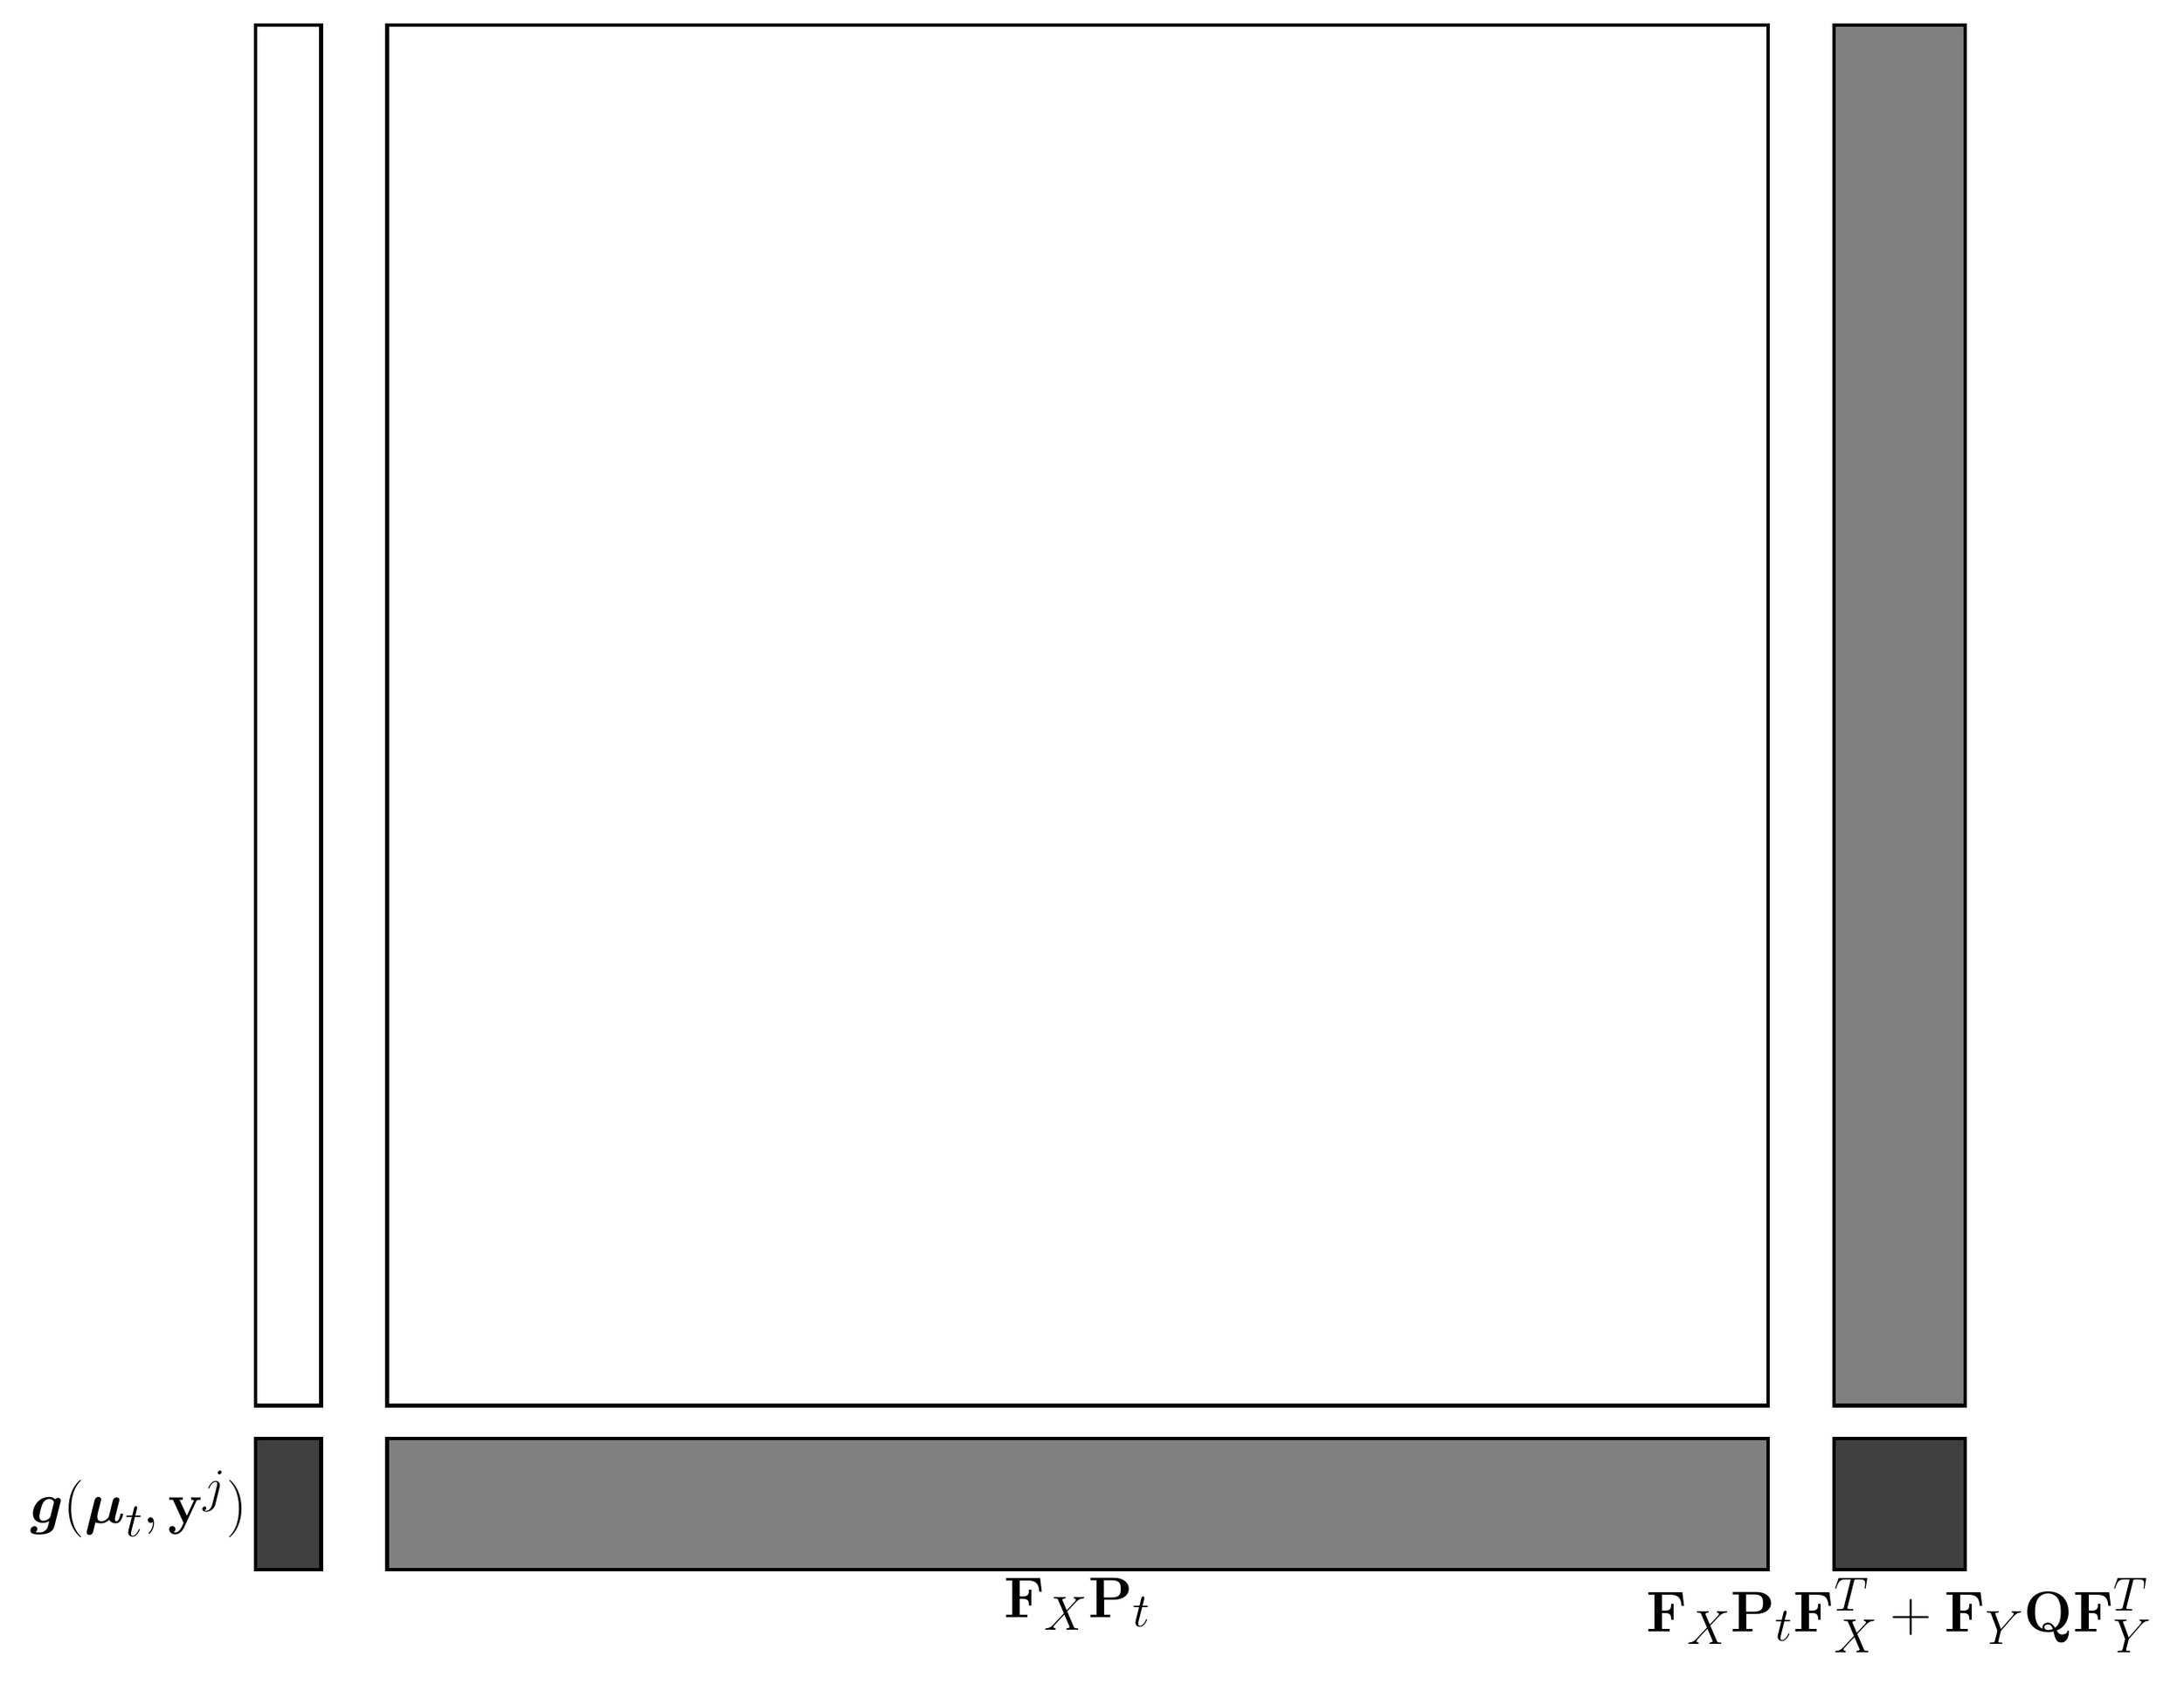
\begin{tikzpicture}
  \tikzmath{\m = 21;}
  \draw[ultra thick] (0, 2.5) rectangle ++(1, \m);
  \draw[ultra thick, fill=darkgray] (0, 0) rectangle ++(1, 2);
  \path (0,0) -- (0, 2) node[midway, anchor=east] {\Huge$\boldsymbol{g}(\boldsymbol{\mu}_t, \mathbf{y}^j)$};


  \draw[ultra thick] (2, 2.5) rectangle ++(\m, \m);
  
  \draw[ultra thick, fill=gray] (2, 0) rectangle ++(\m, 2);
  \path (2,0) -- ++(\m, 0) node[midway, anchor=north] {\Huge$\mathbf{F}_X \mathbf{P}_t$};

  \draw[ultra thick, fill=gray] (2.5+\m+0.5, 2.5) rectangle ++(2, \m);
  \draw[ultra thick, fill=darkgray] (2.5+\m+0.5, 0) rectangle ++(2, 2);
  \path (2.5+\m+0.5, 0) -- ++(2, 0) node[midway, anchor=north] {\Huge$\mathbf{F}_X\mathbf{P}_t\mathbf{F}_X^T + \mathbf{F}_Y\mathbf{Q}\mathbf{F}_Y^T$};
\end{tikzpicture}
\end{document}